% ==============================================================
% EVOLUISM. THREE REFLECTIONS OF ONE REALITY
% Conceptual English Edition — Philosophical Framework
% Linked to Evoluism(S) (Zenodo DOI: 10.5281/zenodo.17454336)
% ==============================================================

\documentclass[11pt,a4paper]{article}

% --- Encoding & fonts
\usepackage[utf8]{inputenc}
\usepackage[T1]{fontenc}

% --- Geometry
\usepackage{geometry}
\geometry{margin=2.5cm}

% --- Math & symbols
\usepackage{amsmath,amssymb}

% --- Graphics & TikZ
\usepackage{graphicx}
\usepackage{tikz}
\usetikzlibrary{positioning,arrows.meta} % for below=of and arrowheads

% --- Hyperlinks
\usepackage{hyperref}
\hypersetup{
  colorlinks=true,
  linkcolor=blue,
  urlcolor=cyan,
  citecolor=black
}

% --- Lists, captions, floats, micro-typography
\usepackage{enumitem}
\usepackage{caption}
\usepackage{float}
\usepackage{microtype}
\usepackage[section]{placeins} % keep floats within their sections
\captionsetup{
  justification=raggedright,
  singlelinecheck=false,
  font=small
}
\setlength{\emergencystretch}{3em} % gentle fix for rare overfull lines

% --- Title
\title{\textbf{EVOLUISM: Three Reflections of One Reality}\\[3pt]
\large Integrating the Metaphysical (M), Philosophical (P), and Scientific (S) Registers}
\author{Evoluit-M \\ \textit{Independent Theoretical Research Evoluism Initiative}}
\date{06 November 2025}

\begin{document}
\maketitle

\begin{abstract}
This paper presents the conceptual foundation of \textit{Evoluism}---a unified framework linking 
metaphysical (M), philosophical (P), and scientific (S) modes of understanding. 
The philosophical idea of Evoluism predates our empirical work; 
the present conceptual article refines its terms, scope, and internal structure. 
It does not continue the empirical research. Rather, it \emph{references and illustrates} 
the empirical findings reported in \textit{Evoluism: Quantifying the Influence of Consciousness on 
Evolutionary Trajectories of Complex Systems} (Zenodo, DOI: \href{https://doi.org/10.5281/zenodo.17454336}{10.5281/zenodo.17454336}, version v2) 
and uses those macro-statistical results (85 countries, 2001--2021; 
$\beta_{\text{synergy}}\!\approx\!0.70$, $p<0.01$) to demonstrate how the scientific register---Evoluism (S)---can 
\emph{operationalize and interpret} the philosophical notions introduced here 
(Source, Flow, Co-Creation). Accordingly, this text states the metaphysical assumptions, 
philosophical principles, and ethical commitments that ground the scientific program, 
while the empirical paper provides one concrete operationalization and test.
\end{abstract}

\noindent This article is archived at Zenodo: \href{https://doi.org/10.5281/zenodo.17547104}{10.5281/zenodo.17547104}

% --------------------------------------------------------------
\section*{Preamble}

This work is neither a scientific article nor a religious declaration.
It is a \textbf{conceptual framework} that seeks to reconcile three complementary ways of knowing reality:
\begin{itemize}[leftmargin=2em]
  \item \textbf{Metaphysical (M)} — seeks meaning and grounding,
  \item \textbf{Philosophical (P)} — reflects on participation and thought,
  \item \textbf{Scientific (S)} — measures and tests action.
\end{itemize}
Evoluism does not claim that these approaches are free from conflict.
It acknowledges their historical tensions and proposes a procedure of productive translation among them:
(i) formulate within one register,
(ii) translate into another with minimal distortion,
(iii) test for coherence and empirical trace,
(iv) return the refined result to the original domain.

% --------------------------------------------------------------
\section{Terminology and Operational Definitions}

For clarity, Evoluism distinguishes metaphorical from operational usage of core terms:

\begin{description}[leftmargin=2em]
\item[Self-unfolding of Reality] The process by which new stable structures arise through interactions among matter, information, and consciousness.
\textit{Operationally:} observed increase of order or functional complexity in systems under continuous input of energy or knowledge.

\item[Coherence (M)] The principle of internal consistency allowing local emergence of order.
\textit{Operationally:} sustained correlations or patterns maintained by flows of energy and information.

\item[Consciousness (P/S)] The ability of a system to model its own state and act upon that model.
\textit{Operationally:} approximated via composite indices of cognitive capital---education, R\&D, and institutional freedom.

\item[``Consciousness as Energy''] Metaphor only.
\textit{Operationally:} increased informational and organizational efficiency---less entropy per achieved goal.
\end{description}

% --------------------------------------------------------------
\section{Definition of Evoluism}

\textbf{Evoluism} (from Latin \textit{ēvolvĕre}---``to unfold'') is the principle that reality develops through
dynamic interactions of \textit{matter}, \textit{information}, and \textit{consciousness},
forming cycles of feedback where form, meaning, and action reinforce one another.

Evoluism synthesizes insights from process philosophy (Whitehead), creative evolution (Bergson),
synergetics (Haken, Prigogine), and complexity theory (Kauffman, Deutsch).
It does not merge science and faith into one discourse but offers a language in which both can coexist without negating each other.

\begin{quote}
Example cycle: biological evolution $\rightarrow$ emergence of mind $\rightarrow$ technology $\rightarrow$ environmental transformation $\rightarrow$ new forms of life and thought.
\end{quote}

% --------------------------------------------------------------
\section{Three Reflections of One Reality}

\subsection*{1. Source — Metaphysical Reflection (M)}
The \textit{Source} denotes the internal principle of coherence enabling ``islands of order'' within an entropic universe.
It is not a deity or substance but the \textit{condition for connected being}.
Evoluism adopts minimal ontological commitment: only \textbf{processes and their local coherence} are assumed to exist; all else are descriptive languages.
Philosophically it resonates with Bergson’s \textit{creative duration} and Whitehead’s \textit{process of becoming};
physically it parallels Prigogine’s dissipative structures sustained by energy and information flows.
\begin{quote}
\textbf{Evoluism-M:} Being is the manifestation of coherence from which form emerges.
\end{quote}

\subsection*{2. Flow — Philosophical Reflection (P)}
\textit{Flow} represents the process of becoming, where consciousness does not mirror the world but participates in it.
Knowledge is not reflection but active engagement.
Higher consciousness correlates with greater synchronization between inner and outer processes, increasing informational efficiency and reducing systemic friction.
\begin{quote}
\textbf{Evoluism-P:} Reality is the mutual participation of consciousness and world, where understanding itself becomes a creative act.
\end{quote}

\subsection*{3. Co-Creation — Scientific Reflection (S)}
\textit{Co-Creation} denotes the empirical manifestation of conscious participation in evolution of complex systems.
Here, consciousness acts as a cognitive feedback loop accelerating systemic development through learning and innovation.

\paragraph{Empirical Foundation and Prediction.}
Based on \textit{Evoluism (S)} dataset (85 countries, 2001--2021; WIPO/OECD/World Bank),
a dynamic panel model of innovation output \(X\) and cognitive capital \(C\) was estimated:
\[
\log(X_{i,t}+1)=\rho\log(X_{i,t-1}+1)+\beta C_{i,t}+\gamma\log(GDP_{i,t})+\alpha_i+\tau_t+\varepsilon_{i,t},
\]
using two-step robust Arellano--Bond GMM.
Result: \(\beta\approx0.70,\,p<0.01\), with valid AR(2) and Hansen tests.
\begin{quote}
\textbf{Prediction:} a +1 SD increase in cognitive capital yields a cumulative rise of $\sim70\%$ in innovation output over 5 years,
holding GDP and demography constant (\textit{Evoluism S}, v1).
\end{quote}
\textbf{Evoluism-S:} Consciousness is an observable driver of accelerated evolution in complex systems through positive cognitive feedback.

% --------------------------------------------------------------
\section{Inter-Level Principles}
Transitions among the three reflections follow three systemic mechanisms:
\begin{enumerate}[label=(\roman*),leftmargin=2em]
  \item \textbf{Emergence:} new properties arise from interactions of micro-systems (physics $\rightarrow$ life $\rightarrow$ cognition);
  \item \textbf{Constraint Transmission:} macro-level institutions and norms reshape micro-behaviors (macro $\rightarrow$ micro);
  \item \textbf{Information Loops:} models of the world alter actions, actions alter environment, environment reshapes models.
\end{enumerate}

% --------------------------------------------------------------
\section{Cycle of Scales and Feedbacks}

\begin{figure}[htbp]
\centering
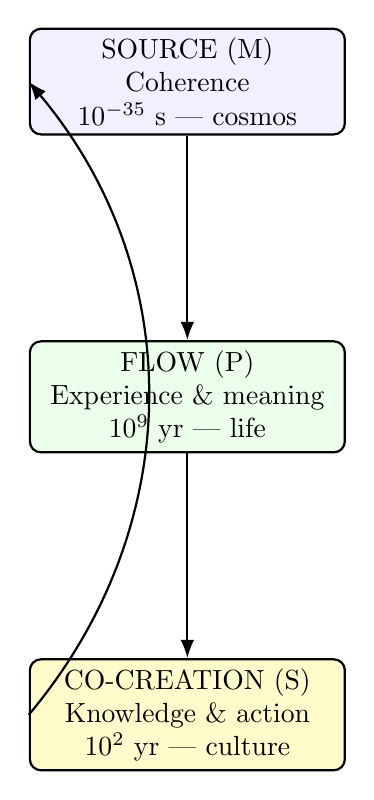
\begin{tikzpicture}[node distance=2.6cm,>=Latex,thick]
\tikzstyle{block}=[rectangle,draw,rounded corners,align=center,minimum width=4.0cm,minimum height=1.25cm]
\node[block,fill=blue!6]   (M) {SOURCE (M)\\Coherence\\$10^{-35}$ s --- cosmos};
\node[block,fill=green!8,below=of M] (P) {FLOW (P)\\Experience \& meaning\\$10^{9}$ yr --- life};
\node[block,fill=yellow!20,below=of P] (S) {CO-CREATION (S)\\Knowledge \& action\\$10^{2}$ yr --- culture};

\draw[->] (M) -- (P);
\draw[->] (P) -- (S);
\draw[->,bend right=40] (S.west) to (M.west);
\end{tikzpicture}

\caption{\parbox{\linewidth}{\textbf{Evoluism cycle} across scales and feedbacks: M $\rightarrow$ P $\rightarrow$ S with a closing feedback S $\rightarrow$ M.}}
\end{figure}

% --------------------------------------------------------------
\section{Process Blocks Diagram (M--P--S)}

\begin{figure}[htbp]
\centering
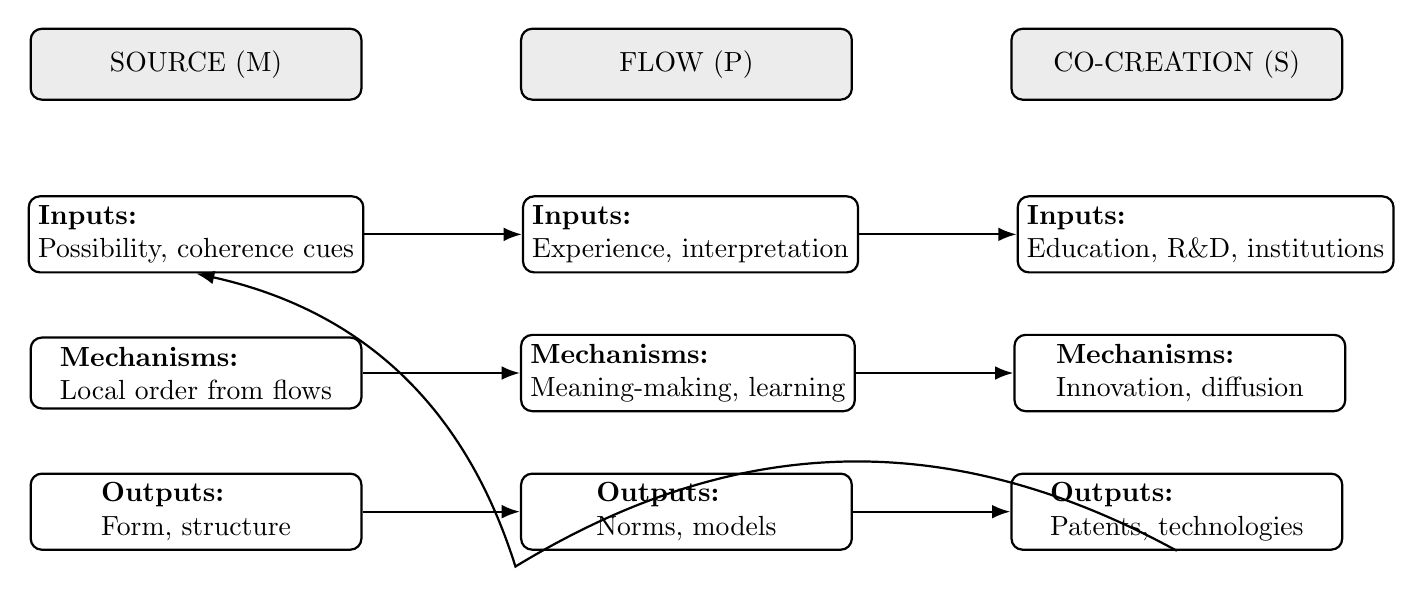
\begin{tikzpicture}[>=Latex,thick,node distance=1.2cm]
\tikzstyle{hdr}=[rectangle,draw,fill=gray!15,rounded corners,align=center,minimum width=4.2cm,minimum height=0.9cm]
\tikzstyle{cell}=[rectangle,draw,rounded corners,align=left,minimum width=4.2cm,minimum height=0.9cm]

% Column headers
\node[hdr] (HM) {SOURCE (M)};
\node[hdr,right=2.0cm of HM] (HP) {FLOW (P)};
\node[hdr,right=2.0cm of HP] (HS) {CO-CREATION (S)};

% Row 1: Inputs
\node[cell,below=of HM] (IM) {\textbf{Inputs:}\\Possibility, coherence cues};
\node[cell,right=2.0cm of IM] (IP) {\textbf{Inputs:}\\Experience, interpretation};
\node[cell,right=2.0cm of IP] (IS) {\textbf{Inputs:}\\Education, R\&D, institutions};

% Row 2: Mechanisms
\node[cell,below=0.8cm of IM] (MM) {\textbf{Mechanisms:}\\Local order from flows};
\node[cell,right=2.0cm of MM] (MP) {\textbf{Mechanisms:}\\Meaning-making, learning};
\node[cell,right=2.0cm of MP] (MS) {\textbf{Mechanisms:}\\Innovation, diffusion};

% Row 3: Outputs
\node[cell,below=0.8cm of MM] (OM) {\textbf{Outputs:}\\Form, structure};
\node[cell,right=2.0cm of OM] (OP) {\textbf{Outputs:}\\Norms, models};
\node[cell,right=2.0cm of OP] (OS) {\textbf{Outputs:}\\Patents, technologies};

% Horizontal flows
\draw[->] (IM.east) -- (IP.west);
\draw[->] (IP.east) -- (IS.west);

\draw[->] (MM.east) -- (MP.west);
\draw[->] (MP.east) -- (MS.west);

\draw[->] (OM.east) -- (OP.west);
\draw[->] (OP.east) -- (OS.west);

% Feedbacks back to M
\draw[->,bend right=30] (OS.south) to ++(-8.4cm,-0.2cm) to (IM.south);
\end{tikzpicture}

\caption{\parbox{\linewidth}{Process blocks for each register (M, P, S): inputs, mechanisms, outputs, and cross-level feedbacks.}}
\end{figure}

% --------------------------------------------------------------
\section{Ethics of Evoluism}
If being is the unfolding of possibilities:
\begin{itemize}[leftmargin=2em]
  \item \textbf{Good} --- actions that enhance coherence, awareness, and sustainable growth;
  \item \textbf{Evil} --- actions that break connections and reduce awareness.
\end{itemize}
\textbf{Ethical principle:} \textit{Act so that through you the Flow continues without breaking the balance of the system.}
Criterion of balance: \textbf{stability under change of scale} and \textbf{capacity for learning and adaptation}.

% --------------------------------------------------------------
\section{Limitations and Open Questions}
\begin{itemize}[leftmargin=2em]
\item Conceptual terms require further operational refinement.
\item Possible reverse causality between innovation and cognitive capital---future work: IV and natural experiments.
\item Macro-level effects may not scale down; micro-validation is planned.
\item The Source is not identified with a theistic God; multiple readings remain admissible.
\end{itemize}

% --------------------------------------------------------------
\section{Continuity Note}
This doctrine provides the philosophical and conceptual framework that 
\emph{contextualizes and supports} the empirical foundation of Scientific Evoluism (Zenodo, 
DOI: \href{https://doi.org/10.5281/zenodo.17454336}{10.5281/zenodo.17454336}, version v2). 
Future research in Evoluism (S) will reference this paper as its philosophical and methodological 
grounding for the continued development of testable models.

% --------------------------------------------------------------
\section{References}
\begin{enumerate}[leftmargin=2em]
\item Whitehead, A. N. (1929). \textit{Process and Reality.}
\item Bergson, H. (1907). \textit{L’Évolution créatrice.}
\item Prigogine, I. (1980). \textit{From Being to Becoming.}
\item Haken, H. (1977). \textit{Synergetics.}
\item James, W. (1912). \textit{Essays in Radical Empiricism.}
\item Dewey, J. (1925). \textit{Experience and Nature.}
\item Merleau-Ponty, M. (1945). \textit{Phénoménologie de la perception.}
\item Kauffman, S. (1995). \textit{At Home in the Universe.}
\item Deutsch, D. (2011). \textit{The Beginning of Infinity.}
\end{enumerate}

\vfill
\noindent
\textbf{License:} CC BY 4.0\\
\textbf{Zenodo DOI:} \href{https://doi.org/10.5281/zenodo.17547104}{10.5281/zenodo.17547104}\\
The complete LaTeX source files, diagrams, and updates are available at:\\
\href{https://github.com/Evoluit-M/Evoluism}{\texttt{https://github.com/Evoluit-M/Evoluism}}\\
\textbf{Author:} Evoluit-M --- \textit{Independent Theoretical Research Evoluism Initiative (2025)}\\
\textbf{Contact:} \href{mailto:evoluit-m@proton.me}{evoluit-m@proton.me}

\end{document}